\section{Définition}
Le pipeline graphique représente la succession des tâches réalisées par la carte graphique dans le but de calculer le rendu d'une scène 3D afin d'afficher celle-ci à l'écran.
\\\\
En entrée, il récupère les informations brutes de la scène 3D :
\begin{itemize}
\item Le type, les coordonnées et la couleur de chaque vertice.
\item Les coordonnées des éventuelles textures à appliquer.
\\
\end{itemize}

En sortie, il renvoie une image 2D composée de pixels.
\\
%\textbf{Le texel} est le plus petit élément d'une texture appliquée à une surface.
\\\\
Le pipeline se décompose en 3 étapes : 
\begin{itemize}
  \item Etape 1 : Transformations et calculs géométriques sur les sommets.
  \item Etape 2 : Pour chaque objet, calcul du rendu local et application des textures.
  \item Etape 3 : Construction (mise à l'échelle) et rendu de l'image finale.\end{itemize}

Source : \cite{pipeline2}
\newpage
\section{Historique}
1998/1999 : La première génération (rastérisation + texture mapping par le GPU)
\\
\begin{center}
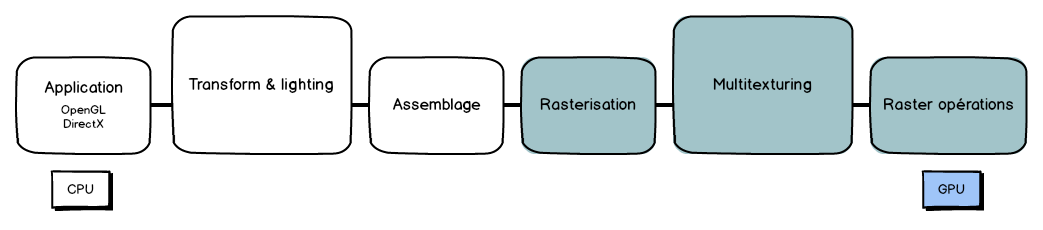
\includegraphics[width=14cm,height=35mm]{pipeline/images/pipeline1.png}
\end{center}
1999/2000 : La deuxième génération (Transform \& lighting par le GPU)
\\
\begin{center}
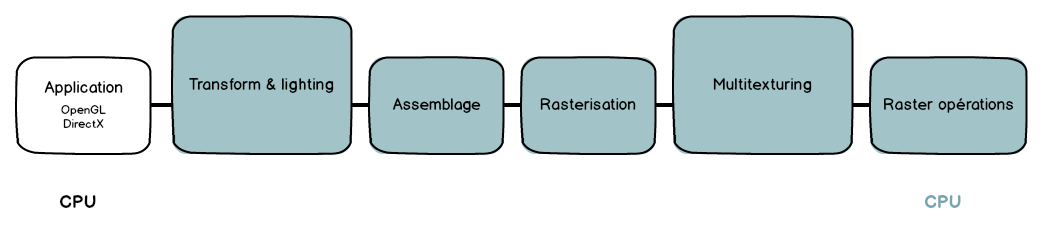
\includegraphics[width=14cm,height=35mm]{pipeline/images/pipeline2.png} 
\end{center}
2001/2002 : Troisième génération (Vertex shader par le GPU)
\\
\begin{center}
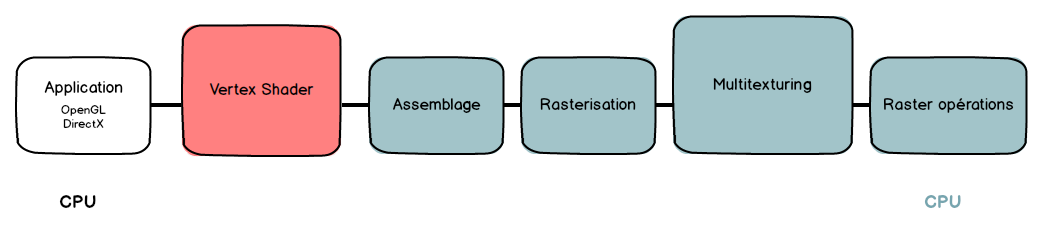
\includegraphics[width=14cm,height=35mm]{pipeline/images/pipeline3.png}
\end{center}
2003 : Quatrième génération (Fragment (ou Pixel) shader par le GPU)
\\
\begin{center}
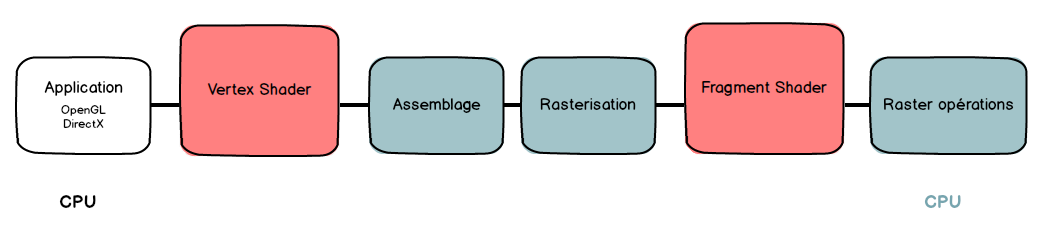
\includegraphics[width=14cm,height=35mm]{pipeline/images/pipeline4.png}
\end{center}

Source : \cite{histoirePipeline}

\section{Deux sortes de pipeline : Fixe (FFP) et dynamique (PFP)}
Le pipeline fixe n'inclut pas l'utilisation de shader. Il n’est donc pas programmable par les développeurs, mais est assez optimisé pour les calculs de toutes les étapes du pipeline.
\\
Au contraire, le pipeline dynamique, et ses shaders nous permettent de définir exactement le rendu à l’écran désiré. La création d’algorithmes qui diffèrent de ceux contenus dans le pipeline fixe, permet des changements au niveau de certains paramètres comme par exemple, les contrastes, les ombres, la lumière, les effets de Cell Shading ou de bump mapping…
\\
Les trois étapes programmables sont donc le vertex shader, le geometry shader, et le fragment shader ou pixel shader.
\\
Un vertex ou vertice, est un sommet d’une figure géométrique (un point particulier d’une figure).

\section{Déroulement du pipeline}
\subsection{Schéma}
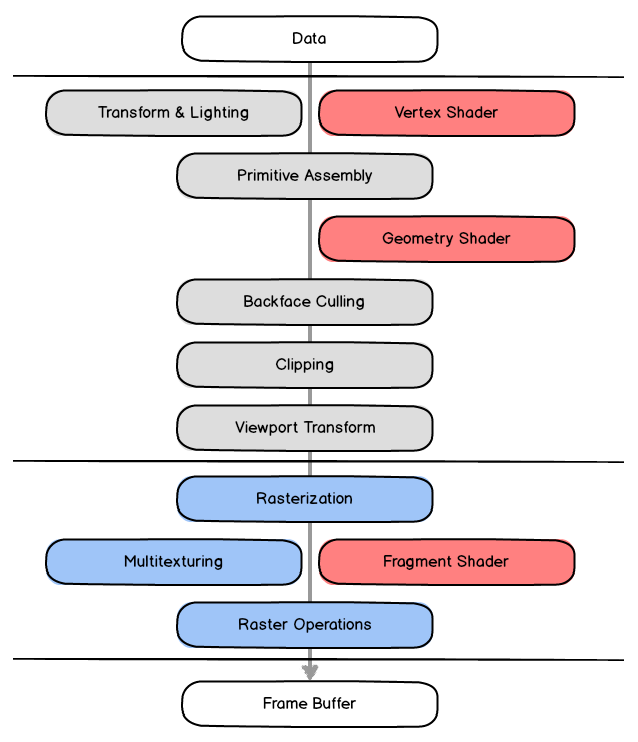
\includegraphics[width=14cm,height=180mm]{pipeline/images/pipeline.png}
Source : \cite{pipeline1}
\newpage
\subsection{Définition des étapes}
\subsubsection{Data (Données brutes)}
Définition des vertices ainsi que leurs coordonnées. Ces données sont enregistrées dans la mémoire de l'ordinateur ou dans un tableau de vertices (Vertex Buffer) sur le GPU suivant la méthode utilisée. L’input assembler est le circuit qui va charger les vertices dans le pipeline à partir de l’adresse de départ du tableau. A la lecture de chaque vertex, celui-ci passe dans le Vertex Cache. Le mémoire cache étant plus rapide, lors des utilisations ultérieures des vertices, la lecture sera plus rapide.
Chaque sommet est déclaré avec ses coordonnées x,y et z. Il peut aussi recevoir une couleur r,g,b,a, une normale Nx, Ny, Nz, une texture u,v, une taille et un poids.
\subsubsection{Transform \& lighting}
Transformation, positionnement et éclairage des sommets en passant du repère local au repère global puis dans l’espace projeté.
\\
Cette tâche peut se décomposer en plusieurs opérations :
\\\\
\textbf{En entrée :} tableaux de coordonnées de sommets dans le repère de l’objet.
\\
\begin{center}
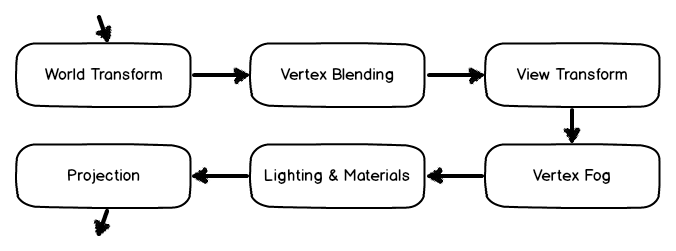
\includegraphics[width=12cm,height=50mm]{pipeline/images/T&L.png}
\end{center}

\textbf{\\En sortie} : sommets avec calculs d’illumination dans l’espace projeté.\\
\begin{itemize}
  \item{\textbf{World Transform}}
Le repère local est le repère affecté à chaque objet. Chaque vertex de l’objet est localisé par rapport au centre de l’objet de coordonnées (0, 0, 0).
\\
\begin{center}
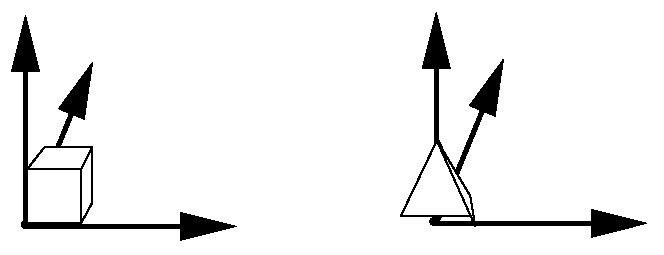
\includegraphics[width=10cm,height=40mm]{pipeline/images/repereLocal.png}
\end{center}

Le passage au repère global qui est le repère de la caméra, ou de l’observateur, s’exécute en changeant les coordonnées de chaque objet, qui passe donc de (0, 0, 0) à (X, Y, Z). Chaque vertice de chaque objet se met à jour en fonction des coordonnées X, Y et Z.
\\
\begin{center}
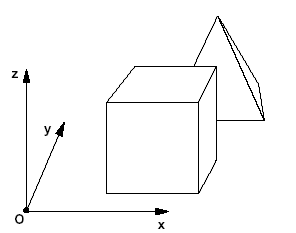
\includegraphics[width=10cm,height=60mm]{pipeline/images/repereGlobal.png}\\
\end{center}

Il faut que l’objet soit dans la bonne orientation, et qu’il soit au bon endroit. Cela peut nécessiter une translation, une rotation ou une mise à l’échelle. Ces opérations peuvent être effectuées sur chaque vertex (X, Y, Z). Les calculs peuvent donc être parallélisés et sont effectués par le GPU. Les calculs de transformation, rotation, et de mise à l’échelle sont des multiplications de ces vertices par des matrices prédéfinies. Chaque opération a une matrice de multiplication prédéfinie, et des matrices existent aussi pour effectuer deux opérations en même temps.
\\
	\item{\textbf{Vertex Blending}}
Combinaison d’un ou plusieurs ensembles de sommets.
\\
	\item{\textbf{View Transform}}
Passage du repère global au repère de la caméra. Après cette transformation, le point de coordonnées (0, 0, 0) sera la caméra. La direction de la vue de l’observateur sera alignée avec l'axe de la profondeur (l'axe Z). La transformation est opérée par le même principe que le "World Transform".
\\
\begin{center}
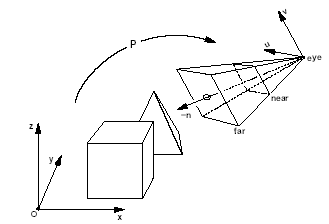
\includegraphics[width=10cm,height=60mm]{pipeline/images/repereCamera.png}
\end{center}

	\item{\textbf{Vertex Fog}}
Calcul de la couleur du brouillard pour chaque sommet.
\\
	\item{\textbf{Lighting \& Materials}}
Chaque vertex fournit des couleurs RGB pour définir comment il réagit à la lumière (réflexion, teinte, contraste…). On lui attribue alors une couleur RGB correspondant à son éclairage.
\\
	\item{\textbf{Projection Transform}}
Passage du repère de l'observateur à l'espace projeté.
\\
\end{itemize}

Source : \cite{pipeline3}

\subsubsection{Primitive assembly ou Tesselation}
Assemblage des vertices sous forme de triangles. L’assemblage s’effectue en prenant les vertices dans l’ordre dans lequel elles sont enregistrées dans la mémoire.
\\\\
Il existe trois méthodes d’assemblage :
\begin{itemize}
	\item Chaque paquet de trois vertex est un triangle indépendant.
	\item Les deux derniers vertex de chaque triangle sont les deux premiers vertex d’un autre triangle (bande de triangle ou triangle strip).
	\item Le premier élément est relié à chaque paire d’élément suivant (Triangle fan).
	\end{itemize}
Décomposer des formes complexes, en formes géométriques simple.

\subsubsection{Backface Culling}
Supprime de l’affichage les triangles qui  tournent le dos à la caméra (face arrière d’une face) en effectuant un calcul avec sa normale.
\subsubsection{Clipping}
Découpe et supprime de l’affichage les parties non visibles des objets partiellement visibles.
\subsubsection{Viewport transform}
Supprime les parties qui ne sont pas dans les coordonnées de l’écran.

\subsubsection{Rasterization}
La rastérisation, ou matricialisation, est composée du triangle setup et de l’interpolation des pixels.
\begin{itemize}
  \item{\textbf{setup ou pixellisation des triangles}} 
Utilisation de la fonction des contours : Renvoi d’un nombre entier (-1, 0, 1) pour chaque pixel en fonction d’une droite. D’un côté de la droite, -1, de l’autre, 1 et sur la droite 0.
En appliquant cette fonction aux trois segments, nous avons :
\begin{itemize}
	\item A l'intérieur du triangle, les trois fonctions (une par côté) donneront un résultat positif.
	\item A l'extérieur, une des trois fonctions donnera un résultat négatif.
\end{itemize}
Si les 3 résultats des fonctions de contours pour un pixel sont positifs, cela veut dire que le pixel appartient au triangle.
L’optimisation de ce procédé est déterminer le plus petit rectangle qui contient le triangle testé, pour exécuter le test des contours seulement sur un nombre de pixels réduit, et non sur tous les pixels de la forme.
Les tests des pixels sont exécutés parallèlement pour un gain de temps.
\item{\textbf{Interpolation}}
Chaque vertex a reçu divers paramètre comme la couleur, la profondeur. Chaque fragment  de chaque triangle, va recevoir en attributs sa couleur, sa profondeur, sa position à l’écran, une valeur de stencil, une transparence, par interpolations des trois vertices définis précédemment.
\end{itemize}
\subsubsection{Multitexturing}
Mélange des textures avec un rendu d’illumination.

\subsubsection{Raster Operations (ROP)}
Cette tâche peut se décomposée en plusieurs opérations :
\\\\
\textbf{En entrée} : Tableau de fragment
\begin{center}
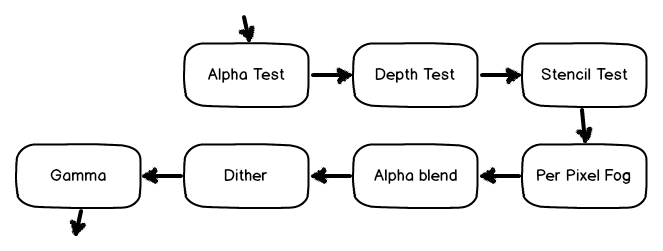
\includegraphics[width=12cm,height=50mm]{pipeline/images/rasterOp.png}
\end{center}
\textbf{\\En sortie} : le pixel prêt à être affiché relativement à l'état courant de traitement du flux de sommets.
\\

\begin{itemize}
	\item{\textbf{Alpha Test}}
C’est le test de transparence. Certaines textures ou couleurs pouvant être transparentes, il faut pouvoir lire le canal alpha d’un pixel. Cette étape supprime tous les pixels qui n’ont pas un alpha acceptable.
\\
	\item{\textbf{Depth Test}}
C’est le test de visibilité (profondeur). C’est la coordonnée z de chaque fragment qui est comparée avec la coordonnée z des autres fragments qui sont sur le même pixel. La carte graphique utilise un depth-buffer qui est un tableau stocké en mémoire. Ce tableau va stocker pour chaque pixel la coordonnée z de l’objet le plus proche de l’écran.
C’est le circuit de gestion de la profondeur qui s’occupe de mettre à jour le depth-buffer. Il va récupérer les coordonnées du fragment reçu à l’écran, puis lire en mémoire la coordonnée z correspondante dans le tableau. Il va comparer celle-ci avec la coordonnée z du fragment reçu, et décider ou non de mettre à jour le depth-buffer et le frame-buffer.
Il faut que ces coordonnées z soient codées sur assez de bits pour avoir une bonne précision, et ne pas se retrouver avec des artefacts visuels.
\\
	\item{\textbf{Stencil Test}}
Un stencil est en  français un pochoir. C’est une sorte de masque que l’on affiche sur l’écran pour définir une vue restreinte comme une vue à travers un hublot, ou une serrure.
\\
	\item{\textbf{Per-pixel Fog}}
Cette étape permet de rajouter du brouillard (≠phénomène météorologique) sur chaque pixel. Le brouillard est ajouté grâce à une couleur de brouillard, qui est mélangée avec la couleur du pixel (moyenne). Le brouillard dépend de la profondeur du pixel. Si l’objet est proche, aucun brouillard n’est appliqué, si l’objet est trop loin, c’est seulement la couleur du brouillard qui est affiché.
\\
	\item{\textbf{Alpha Blend}}
Cette tâche sert à calculer la couleur finale du pixel. Notre GPU contient un color buffer, un tableau qui sert à stocker pour chaque pixel sa couleur finale.
Le calcul est simple, à chaque fragment envoyé :
\begin{itemize}
	\item Lecture de l’ancienne couleur du pixel,
	\item Calcul de la couleur finale en fonction du fragment envoyé et de l’ancienne couleur,
	\item Enregistrement du résultat.
\end{itemize}
Les opérations "alpha test" et "alpha blend" sont effectuées par un circuit spécialisé : le Color ROP. Il travaille en parallèle des autres tâches.
\\
	\item{\textbf{Dither}}
Mélange des couleurs des pixels adjacents pour obtenir une couleur plus consistante.
\\
	\item{\textbf{Gamma}}
Applique la correction gamma définie.
\end{itemize}

Source : \cite{pipeline4}

\subsubsection{Framebuffer}
Affichage du résultat à l’écran utilisant le double-buffering, color buffer, Z-buffer.

\subsection{Fonctionnement simple}
\begin{center}
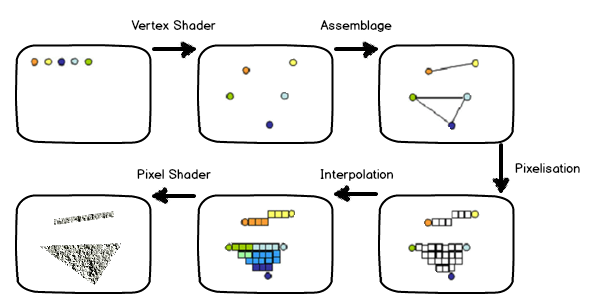
\includegraphics[width=12cm,height=60mm]{pipeline/images/pipelineSimple.png}
\end{center}